\documentclass{article}

\usepackage{amsmath,amssymb}
\usepackage{tikz}
\usepackage{pgfplots}
\usepackage{xcolor}
\usepackage[left=2.1cm,right=3.1cm,bottom=3cm,footskip=0.75cm,headsep=0.5cm]{geometry}
\usepackage{enumerate}
\usepackage{enumitem}
\usepackage{marvosym}
\usepackage{tabularx}
\usepackage{parskip}

\usepackage{listings}
\definecolor{lightlightgray}{rgb}{0.95,0.95,0.95}
\definecolor{lila}{rgb}{0.8,0,0.8}
\definecolor{mygray}{rgb}{0.5,0.5,0.5}
\definecolor{mygreen}{rgb}{0,0.8,0.26}
%\lstdefinestyle{java} {language=java}
\lstset{language=R,
	basicstyle=\ttfamily,
	keywordstyle=\color{lila},
	commentstyle=\color{lightgray},
	stringstyle=\color{mygreen}\ttfamily,
	backgroundcolor=\color{white},
	showstringspaces=false,
	numbers=left,
	numbersep=10pt,
	numberstyle=\color{mygray}\ttfamily,
	identifierstyle=\color{blue},
	xleftmargin=.1\textwidth, 
	%xrightmargin=.1\textwidth,
	escapechar=§,
	%literate={\t}{{\ }}1
	breaklines=true,
	postbreak=\mbox{\space}
}

\usepackage[colorlinks = true, linkcolor = blue, urlcolor  = blue, citecolor = blue, anchorcolor = blue]{hyperref}
\usepackage[utf8]{inputenc}

\renewcommand*{\arraystretch}{1.4}

\newcolumntype{L}[1]{>{\raggedright\arraybackslash}p{#1}}
\newcolumntype{R}[1]{>{\raggedleft\arraybackslash}p{#1}}
\newcolumntype{C}[1]{>{\centering\let\newline\\\arraybackslash\hspace{0pt}}m{#1}}

\newcommand{\E}{\mathbb{E}}
\DeclareMathOperator{\rk}{rk}
\DeclareMathOperator{\Var}{Var}
\DeclareMathOperator{\Cov}{Cov}

\title{\textbf{Finanzderivate und Optionen, Übung 3}}
\author{\textsc{Henry Haustein}}
\date{}

\begin{document}
	\maketitle
	
	\section*{Aufgabe 1}
	Richtig, derjenige, der mir den Future verkauft, muss bei der Cash-and-Carry-Strategie komplett in Vorkasse gehen und ich bezahle ihm später alle Kosten.

	\section*{Aufgabe 2}
	Richtig: Der implizite Refinanzierungssatz (\textit{implied repo rate}, IRR) bezieht sich auf die Rendite, die durch den Kauf eines Kassainstruments mit geliehenem Geld bei gleichzeitigem Verkauf eines Futures erzielt werden kann (d.h. impliziert wird).
	
	\section*{Aufgabe 3}
	Der Margin Call kommt dann, wenn die Maintenance Margin nicht mehr ausreicht, um die Kursänderung $\Delta$ abzudecken. Also dann, wenn $\Delta\cdot 5000 > (4000-3000)$, damit $\Delta > 0.2$. Wenn der Kurs also auf über \$17.40 pro Unze steigt, führt das zu einer Nachschussforderung. Wenn man dieser nicht nachkommt, wird die hinterlegte Margin genutzt, um den Kontrakt glattzustellen.
	
	Initial Margin deckt das Marktrisiko und das Liquiditätsrisiko ab. Maintenance Margin wird benötigt, um die Position aufrecht zu erhalten.
	
	Die Variation Margin ist die regelmäßig abgerechnete Margin und stellt den aktuellen Gewinn und Verlust der Position dar.
	
	\section*{Aufgabe 4}
	$\text{Gewinn} = (70.50 - 68.30)\cdot 1000 = 2200$. Dieser Gewinn wird im März 2019 realisiert.
	
	Bis zum 31.12. ist die P/L des Kontraktes $(69.10 - 68.30)\cdot 1000 = 800$. Von dann bis März 2019 ist der Gewinn $2200 - 800 = 1400$ Dollar.
	
	Ein Absicherer müsste im Jahr 2019 den Gesamtgewinn versteuern (\textit{Hedge Accounting}), weil er auch das Underlying besitzt. Ein Spekulant versteuert im Jahr 2018 die \$800, im Jahr 2019 die \$1400.
	
	\section*{Aufgabe 5}
	Forward: privater Vertrag zwischen 2 Parteien, OTC, nicht standardisiert \\
	Future: Handel an der Börse, standardisiert
	
	Forward-Kurs: 1.25 CHF = 1 USD, das ist äquivalent zu 1 CHF = 0.8 USD \\
	Future-Kurs: 1 CHF = 0.798 USD
	
	Wenn ich Franken verkaufen will, dann sollte ich das im Forward machen, da gibt es mehr Dollar dafür.
	
	\section*{Aufgabe 6}
	Richtig, ich kaufe Futures-Kontrakte und, um das Geld später zu haben und die Cost-of-Carry zu bezahlen (die nur Finanzierungkosten enthält), lege ich das Geld auf einem Konto an.
	
	\section*{Aufgabe 7}
	\begin{enumerate}[label=(\alph*)]
		\item \textcolor{green}{Initial Margin}
		\item \textcolor{green}{Kontraktgröße des Futures}
		\item \textcolor{red}{Open Interest des entsprechenden Future-Kontraktes}: Wie viele Futures offen sind, also noch nicht geliefert. Das ist ein Maß für die Liquidität im Markt.
		\item \textcolor{red}{Transaktionskosten für das Kassa- bzw. das Future-Geschäft}
	\end{enumerate}
	
	\section*{Aufgabe 8}
	Der Terminkurs sollte $\text{Kassakurs} + \text{Cost-of-Carry}$ sein:
	\begin{align}
		\text{Terminkurs} &= 200 + (9 - 8.5) \notag \\
		&= 200.5 \notag
	\end{align}
	Der Future am Markt ist zu billig, ich sollte diesen also kaufen und das Underlying verkaufen (Reverse-Cash-and-Carry).
	
	\section*{Aufgabe 9}
	Analog zu Aufgabe 8 sollte hier der Terminkurs
	\begin{align}
		\text{Terminkurs} &= 96 + (2 - 4) \notag \\
		&= 94 \notag
	\end{align}
	Hier ist der Future am Markt zu billig, ich sollte diesen also kaufen und das Underlying verkaufen (Reverse-Cash-and-Carry).
	
	\section*{Aufgabe 10}
	Der Unterschied zwischen den Mittelzuflüssen (Erträge) und Mittelabflüssen (Aufwendungen) eines Basiswertes wird als Haltekosten/Basis oder Cost-of-Carry bezeichnet.
	
	\section*{Aufgabe 11}
	\begin{center}
		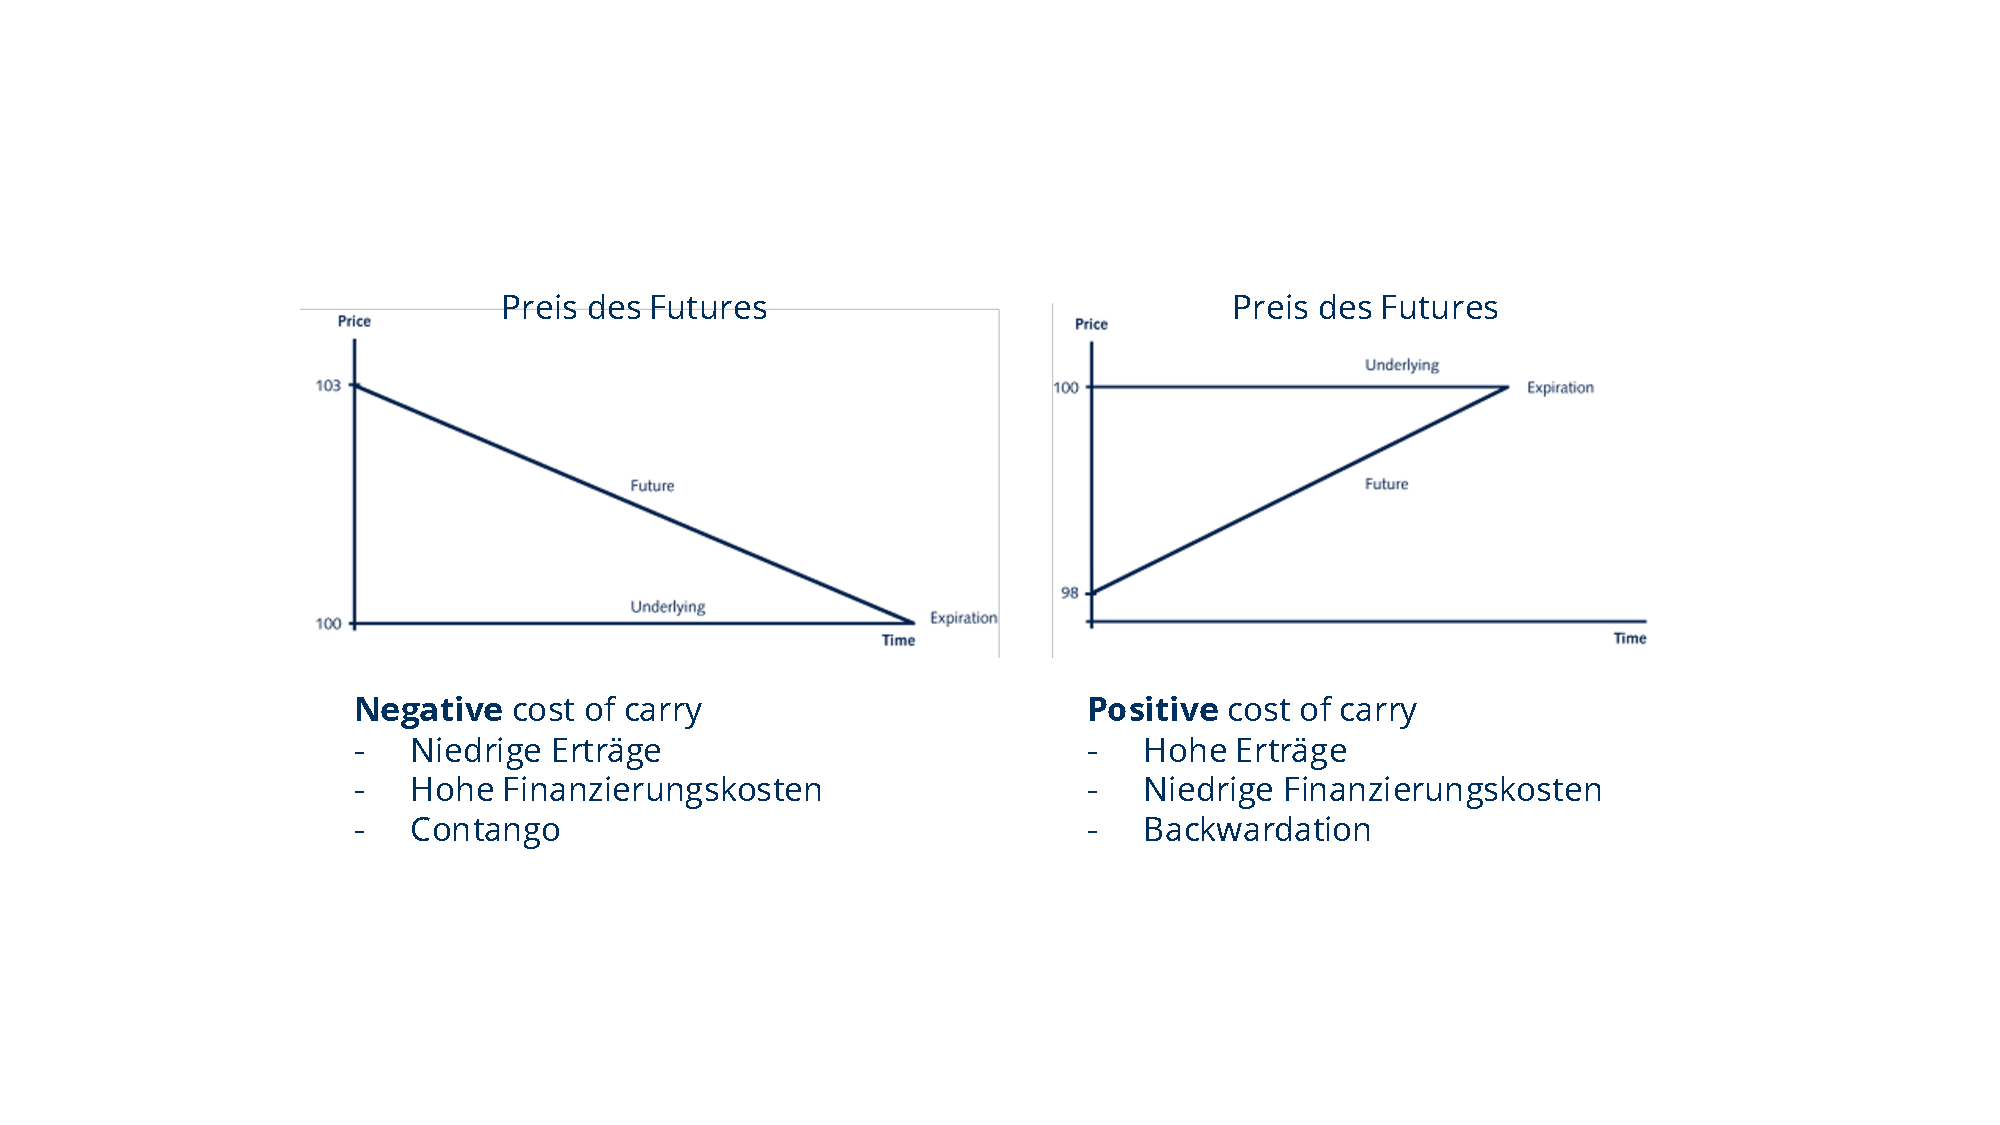
\includegraphics[scale=0.5]{Aufgabe 3.11}
	\end{center}
	
	\section*{Aufgabe 12}
	Backwardation: positive cost of carry \\
	Contango: negative cost of carry
	
	\section*{Aufgabe 13}
	Die Basis am 1.10. ist $130-140 = -10$, am 10.10. ist sie $120-135 = -15$, damit hat sich die Basis ausgeweitet (\textit{widening}). Da die Basis negativer wird, spricht man auch von \textit{weakinging}.
	
	\section*{Aufgabe 14}
	Jetzige Basis: $130-140 = -10$, erwartete Basis z.B. -5. Damit sollte der Kassakurs sich erhöhen und der Terminkurs sich verringern. Wir kaufen also Kassa und verkaufen Future.
	
	\section*{Aufgabe 15}
	Falsch, wenn Finanzierungskosten unter den Erträgen liegen, dann handelt es sich um eine positive Cost-of-Carry.
	
	\section*{Aufgabe 16}
	\begin{itemize}
		\item Cash-and-Carry: Long Kassamarkt + short Future, das ist das selbe wie einfach Geld am Geldmarkt anzulegen
		\item Reverse-Cash-and-Carry: Short Kassamarkt + long Future, das ist das selbe wie einen Kredit aufnehmen
		\item Conversion: das selbe wie Cash-and-Carry, nur mit synthetischem Future (short Future = short Call + long Put)
		\item Reversal: das selbe wie Reverse-Cash-and-Carry, nur mit synthetischem Future (long Future = long Call + short Put)
	\end{itemize}
	
	\section*{Aufgabe 17}
	Richtig, siehe Aufgabe 8 und 9.
	
	\section*{Aufgabe 18}
	Kauf des Futures für 113, Verkauf des Underlyings für 106
	\begin{align}
		\frac{113}{1+r} &= 106 \notag \\
		r &= 0.0660 \notag
	\end{align}
	
	\section*{Aufgabe 19}
	Falsch, das Risiko ist, dass man jeden Tag Liquidität haben muss, um die eventuell anfallende Variation Margin zu bezahlen.
	
	\section*{Aufgabe 20}
	Falsch, es gibt Kontraktgrößen und die Margin. Das ist eigentlich das Geld, was man einsetzt.
	
\end{document}